%===============================================================================
% ifacconf.tex 2022-02-11 jpuente  
% 2022-11-11 jpuente change length of abstract
% Template for IFAC meeting papers
% Copyright (c) 2022 International Federation of Automatic Control
%===============================================================================
\documentclass{ifacconf}

% \usepackage{hyperref}
\usepackage{graphicx}      % include this line if your document contains figures
\usepackage{natbib}        % required for bibliography
\usepackage{comment}
\usepackage{amsmath}
\usepackage{amssymb}
\usepackage[dvipsnames]{xcolor}

\usepackage{subfig}
\usepackage{kotex}
\usepackage{tikz}

\usepackage{lipsum} % for dummy text
\usepackage{multirow}
\usepackage{multicol}

\usepackage{algorithm}
\usepackage{algpseudocode}

\usepackage{xurl}

% ============================================
%         GENERAL MACROS
% ============================================
\newcommand{\template}{template}
\newcommand{\KHCH}[1]{{\color{RoyalPurple} [KH: #1]}} % Kyunghwan's
\newcommand{\JYKI}[1]{{\color{red} [JY: #1]}} % Jiyun's
\newcommand{\MSRY}[1]{{\color{Peach} [MS: #1]}} % Myeongseok's 
\newcommand\eg{\textrm{e.g.,\ }}
\newcommand\ie{\textrm{i.e.,\ }}
\definecolor{my_cyan}{rgb}{0.0, 1.0, 1.0}

\newcommand{\colorLine}[2]{[\tikz[baseline=(current bounding box.base)]{\draw[color=#1,
#2,line width=2pt] (0,3pt) -- (1.5em,3pt);}]}
% colors
% https://latexcolor.com % color list
\definecolor{airforceblue}{rgb}{0.36, 0.54, 0.66}
\definecolor{awesome}{rgb}{1.0, 0.13, 0.32}
\newcommand{\ctxt}[2]{{\color{#1}{#2}\color{black}}}
\newcommand{\cred}[1]{{\ctxt{awesome}{#1}}}
\newcommand{\cblue}[1]{{\ctxt{airforceblue}{#1}}}

\begin{comment}
L2 Norm of Tracking Error:
C1: 2.0486
C2: 1.6893
C3: 6.8005
Improvement over C3:
C1: 69.88 %
C2: 75.16 %
\end{comment}

\newcommand{\oneErr}{{2.0486}}
\newcommand{\twoErr}{{1.6893}}
\newcommand{\threeErr}{{6.8005}}

\newcommand{\impOne}{{69.88}}
\newcommand{\impTwo}{{75.16}}

% ============================================
%         MATH MACROS
% ============================================
% \input{\template/macros/macros_math.tex}
\newcommand\R{\mathbb{R}}
\newcommand\N{\mathbb{N}}

\newcommand*{\mv}[1]{\boldsymbol{#1}} % my vector
\newcommand*{\mm}[1]{\boldsymbol{#1}} % my matrix
\newcommand*{\norm}[1]{\lVert #1 \rVert} % euclidean norm

\DeclareMathOperator{\myvec}{{vec}}       % vectorization
\DeclareMathOperator{\myproj}{{Proj}}   % projection
\DeclareMathOperator{\mysat}{{sat}}       % saturation
\DeclareMathOperator{\myrow}{{row}}       % row of a matrix
\DeclareMathOperator{\mycol}{{Col}}       % column of a matrix
\DeclareMathOperator{\mysym}{{sym}}       % symmetric part of a matrix
\DeclareMathOperator{\mydiag}{{diag}}     % diagonal matrix
\DeclareMathOperator{\mysign}{{sign}}     % sign function
\DeclareMathOperator{\mypoly}{{Poly}}     % polynomial

% ============================================
%         FRACTIONS
% ============================================
\newcommand\der{\mathrm d}
\newcommand*{\ddt}{
   \frac{\der}{\der t}
}
\newcommand*{\ddtt}{
   \tfrac{\der}{\der t}
}
\newcommand*{\ddttddtt}{
   \tfrac{\der^2}{\der t^2}
}
\newcommand*{\ddfrac}[2]{
   \frac{\der {#1}}{\der {#2}}
}
\newcommand*{\ddtfrac}[2]{
   \tfrac{\der {#1}}{\der {#2}}
}
\newcommand*{\ppfrac}[2]{
   \frac{\partial {#1}}{\partial {#2}}
}
\newcommand*{\pptfrac}[2]{
   \tfrac{\partial {#1}}{\partial {#2}}
}

%===============================================================================
\begin{document}
\begin{frontmatter}

\title{
   Vector-Space Optimization for Contraction Theory-Based Control Design: An Energy-Based Effective Space Approach
   \thanksref{footnoteinfo}
} 
% Title, preferably not more than 10 words.

\thanks[footnoteinfo]{
   This work was supported in part by the National Research Foundation of Korea (NRF) grant funded by the Korea government (MSIT) (RS-2025-00554087)
}

\author[First]{Myeongseok Ryu} 
\author[First]{Kyunghwan Choi} 
\author[Second]{Sesun You}

\address[First]{
   Korea Advanced Institute of Science and Technology (KAIST), 
   Daejeon 34051, South Korea (e-mail: \{dding\_98, kh.choi\}@kaist.ac.kr)}
\address[Second]{
   Keimyung University, 
   Daegu 42601, South Korea (e-mail: yousesun@kmu.ac.kr)}

\begin{abstract}                % Abstract of 50--100 words
   In this paper, we propose a novel vector-space optimization framework for contraction theory-based control design with input saturation.
   Conventional Linear Matrix Inequality (LMI) optimization frameworks suffer from computational complexity issues for high-dimensional systems and limited flexibility in handling various constraints, including input saturation.
   Moreover, there exists ill-posed problem in the objective function minimizing the condition number of the contraction metric.
   To address these issues, we project the contraction metrics onto the trajectory error vector space, leading to a simplified vector-space optimization framework within a lower-dimensional effective space.
   Furthermore, energy-based constraints are incorporated to obtain a finite number of locally optimal solutions and to maintain sufficient control effort.
   In addition, convex input saturation constraints are integrated to handle the practical limitations of actuators.
   The effectiveness and feasibility of the proposed method are validated through numerical simulations using the Lorenz system.
\end{abstract}

\begin{keyword}
   Contraction theory, 
   optimization-based control,
   input saturation, 
   energy-based control
\end{keyword}

\end{frontmatter}
%===============================================================================

\section{Introduction}

\subsection{Motivation}

Besides the traditional Lyapunov stability theory, contraction theory offers an interesting perspective on the stability analysis of nonlinear systems.
It allows us to analyze system stability by examining the convergence of trajectories rather than the convergence of states to a specific equilibrium point \cite{LOHMILLER:1998aa}.
For this analysis, the differential dynamics of the system are considered to find a Riemann metric, called a contraction metric, which guarantees that all trajectories exponentially converge to a unique trajectory.
One of the advantages of contraction theory-based approaches is that Linear Matrix Inequalities (LMIs) can be used to efficiently obtain global optimal contraction metrics, utilizing the differential nature of contraction theory \cite{Andrieu:2019aa,Manchester:2014aa}.
Additionally, Linear Time-Varying (LTV) system analysis techniques can be applied to design feedback controllers using the contraction metric as a feedback gain \cite{Tsukamoto:2019aa}.

Among recent developments in contraction theory-based control, Tsukamoto {\etal} proposed ConVex optimization-based Steady-state Tracking Error Minimization (CV-STEM), which systematically calculates the contraction metrics in an LMI optimization problem \cite{Tsukamoto:2019aa} to minimize the steady-state tracking error bound in the presence of bounded disturbances.
CV-STEM has demonstrated its effectiveness and has been extended to various systems, including stochastic systems \cite{Tsukamoto:2021ad} and uncertain systems \cite{Tsukamoto:2021af}.

However, since the LMI framework requires matrix-space optimization, the computational complexity increases with respect to the system dimension, as the number of optimization variables is proportional to the square of the system dimension \cite{Boyd:2004aa}.
This makes real-time implementation difficult for high-dimensional systems.
To resolve this, CV-STEM has been combined with deep neural networks (DNNs) to approximate the contraction metrics off-line and implement them in real-time \cite{Tsukamoto:2021ae,Tsukamoto:2021ac}.
For practical real-time implementation, however, it is desirable to reduce the computational complexity of the contraction metric calculation without relying on DNNs.

Moreover, there has been limited consideration of input saturation in conventional contraction theory-based control design, which limits the practical applicability of the method.
For instance, in \cite{Tsukamoto:2019aa}, the input saturation constraint is considered in a conservative manner by limiting the maximum norm of the control input, rather than directly incorporating the contraction metric into the LMI framework.
This may lead to the infeasibility of the optimization problem when the input saturation constraint is tight.
In addition, if the input saturation effect is not properly handled, the system performance may degrade significantly or even become unstable \cite{Ryu:2025aa}.

There is also the issue of an ill-posed problem in the objective function minimizing the condition number of the contraction metric, which is proportional to the steady-state error bound.
Since the condition number is scale-invariant, there exist an infinite number of solutions for the contraction metric that yield the same condition number.
In conventional approaches, this issue has been tackled by introducing a scaling parameter for the contraction metric and tuning it with weighting factors in the objective function \cite{Tsukamoto:2019aa,Tsukamoto:2021ae}.
However, this approach may determine insufficient control effort to achieve the desired trajectory or lead to excessive control effort.

On the other hand, by formulating the problem in vector space rather than matrix space, flexibility in handling various constraints, including nonlinear input and state constraints, can be improved.
In addition, the dependency of computational complexity on the system dimension can be alleviated.
If the contraction metric is utilized as a feedback gain for the trajectory error, the contraction metric can be projected onto the trajectory error vector space.
This allows us to simplify the contraction metric calculation from matrix-space optimization to vector-space optimization within a lower-dimensional effective space.

To the best of our knowledge, there has been no previous work that projects the contraction constraints onto a vector space to reduce the dependency on the system dimension for contraction metric calculation.
Moreover, input saturation has not been actively considered in conventional contraction theory-based control design.
Hence, the main objective of this paper is to simplify the contraction metric calculation from matrix-space optimization to vector-space optimization, while also incorporating the input saturation constraint and maintaining sufficient control effort.

\subsection{Contributions}

The main contributions of this paper are:
\begin{itemize}
   \item The contraction metrics can be calculated in a lower-dimensional effective space by projecting the contraction constraints onto the trajectory error vector space. This significantly reduces the computational complexity of the LMI framework for contraction metric calculation, enabling real-time implementation;
   \item The scale-invariance issues of the objective function minimizing the condition number of the contraction metric are resolved by introducing energy-based constraints to obtain locally optimal solutions and maintain sufficient control effort;
   \item A convex input saturation constraint is incorporated into the proposed optimization framework, which handles the practical limitations of actuators; and
   \item The robust feasibility of the proposed method is enhanced by introducing slack variables to relax the energy-based constraints, thereby avoiding infeasibility due to the input saturation constraint.
\end{itemize}

\subsection{Paper Organization}

The remainder of this paper is organized as follows.
Section \ref{sec:preliminaries} reviews the preliminaries of contraction theory.
Section \ref{sec:problem} formulates the problem of contraction theory-based control design with input saturation.
Section \ref{sec:conv:lmi} discusses the conventional LMI framework for contraction metric calculation and its limitations.
Section \ref{sec:main:results} presents the proposed vector-space optimization framework for contraction metric calculation and provides an illustrative example.
Section \ref{sec:validation} validates the proposed method through numerical simulations.
Finally, Section \ref{sec:conclusion} concludes the paper.

\section{Preliminaries} \label{sec:preliminaries}

Before presenting the proposed method, we first review contraction theory and related theorems.
A detailed explanation of contraction theory can be found in \cite{LOHMILLER:1998aa,Tsukamoto:2021aa}.

\subsection{Contraction Property and Contraction Metric} \label{sec:sub:contraction}

Consider the following nonlinear system:
\begin{equation} \label{eq:pre:sys}
   \ddtt\mv{x}
   =
   \mv{f}(\mv{x},t)
   ,
\end{equation}
where $\mv{x}\in\R^n$ denotes the state variables and $\mv{f}:=\mv{f}(\mv{x},t)$ denotes the nonlinear system function.
Additionally, consider the differential dynamics of the system \eqref{eq:pre:sys}, which is represented as 
$
   \ddtt{\delta\mv{x}}
   =
   \pptfrac{\mv{f}}{\mv{x}} \delta\mv{x}
$
, \cite[Chap 4]{Kirk:2004aa}.

According to \cite{LOHMILLER:1998aa}, the system \eqref{eq:pre:sys} is said to be \textit{contracting}, \ie all trajectories converge incrementally exponentially to a unique trajectory, if the following condition holds:
\begin{equation} \label{eq:pre:contraction:condition}
   \ddtt\mm{M} 
   + 
   2\mysym
   \left(
      \mm{M} \pptfrac{\mv{f}}{\mv{x}}
   \right) 
   \preceq 
   -2\alpha\mm{M}
   ,
\end{equation}
where $\mm{M}$ denotes the \textit{contraction metric}, $\alpha\in\R_{>0}$ denotes the \textit{contraction rate}, and $\mysym(\mm A):=\tfrac{1}{2}(\mm A+\mm A^\top)$.
The contraction metric $\mm{M}$ is a symmetric positive definite matrix satisfying $\overline{m}\mm{I}_n\succeq\mm{M}\succeq\underline{m}\mm{I}_n$ with $\overline{m},\underline{m}\in\R_{>0}$.

Notably, the initial conditions are exponentially forgotten in a contracting system \cite{LOHMILLER:1998aa}.

\subsection{Perturbed Contracting System} \label{sec:sub:contraction:perturbed}

If the system \eqref{eq:pre:sys} is subjected to bounded disturbances, it can be expressed as follows:
\begin{equation} \label{eq:pre:sys:perturbed}
   \ddtt\mv{x}
   =
   \mv{f}(\mv{x},t)
   +
   \mv{d}(t)
   , 
\end{equation}
where $\mv{d}(t)\in\R^n$ denotes the external disturbances with $\norm{\mv{d}(t)}\leq \overline{d}$, where $\overline{d}\in\R_{>0}$.

The following theorem states that all solutions of the perturbed system \eqref{eq:pre:sys:perturbed} exponentially converge to a bounded ball around the solution of the nominal system \eqref{eq:pre:sys}.
\begin{thm} \label{thm:contraction:perturbed}
   If the system \eqref{eq:pre:sys} is contracting with the contraction metric $\mm{M}$ satisfying the condition \eqref{eq:pre:contraction:condition}, the path integral $V_l(\mv{q},\delta\mv{q},t)=\int_{\mv{\xi}_1}^{\mv{\xi}_2}\norm{\mm{\Theta}(\mv{q},t)\delta\mv{q}}$, where $\mm{\Theta}(\mv{q},t):=\mm{M}^{1/2}$, and $\mv{\xi}_1$ and $\mv{\xi}_2$ are the solutions of \eqref{eq:pre:sys} and \eqref{eq:pre:sys:perturbed}, respectively, and $\mv{q}$ is the virtual state variable, exponentially converges to a bounded ball. 
   Specifically, the following inequality for a bounded error ball of the solutions of \eqref{eq:pre:sys} and \eqref{eq:pre:sys:perturbed} holds:
   \begin{equation}
      \norm{\mv\xi_1(t)-\mv\xi_2(t)}
      \le
      \tfrac{V_{l}(0)}{\sqrt{\underline{m}}}
      \exp(-\alpha t)
      +
      \tfrac{\overline d}{\alpha}
      \sqrt{\chi}
      (1-\exp(-\alpha t))
      ,
   \end{equation}
   where $\chi:=\overline{m}/\underline{m}$ denotes the condition number of $\mm{M}$, yielding a steady-state error bound of $\tfrac{\overline d}{\alpha}\chi$.
\end{thm}

\begin{pf}
   See the proof of Theorem 2.4 in \cite{Tsukamoto:2021aa}.
\end{pf}

\section{Problem Formulation} \label{sec:problem}

Let us consider the following nonlinear system:
\begin{equation} \label{eq:sys}
   \begin{aligned}   
      \ddtt{\mv{x}}
      =&
      \mv{f}(\mv{x},t)
      +
      \mm{B}(\mv{x},t)
      \mysat(\mv{u})   
      +
      \mv{d}(t)
      ,
   \end{aligned}
\end{equation}
where $\mv{x}\in\R^n$ and $\mv{u}\in\R^m$ denote the state variables and control inputs, respectively; $\mv{d}:=\mv{d}(t)\in\R^n$ denotes the bounded external disturbances, \ie $\norm{\mv{d}} \leq \overline{d}$; and $\mv{f}(\mv{x},t)$ and $\mm{B}(\mv{x},t)$ denote the system functions.
The input saturation function is denoted by $\mysat(\cdot)$ and can be defined as any physically feasible convex function.

We assume that a desired control input $\mv{u}_d\in\R^m$ is pre-designed to achieve the desired trajectory $\mv{x}_d\in\R^n$ under ideal conditions, \ie $\mv{d}=0$, by simulating the following desired system:
\begin{equation} \label{eq:sys:desired}
   \ddtt\mv{x}_d   =
   \mv{f}(\mv{x}_d, t)   
   +
   \mm{B}(\mv{x}_d,t) \mv{u}_d
   .
\end{equation}

The error dynamics between the system \eqref{eq:sys} and the desired system \eqref{eq:sys:desired} can be expressed as follows:
\begin{equation} \label{eq:error:dyn:1}
   \begin{aligned}
      \ddtt\mv{e}
      =&
      \mv{f}-\mv{f}_d
      + \mm{B} \mysat(\mv{u})
      - \mm{B}_d \mv{u}_d
      + \mv{d}
      ,
   \end{aligned}
\end{equation}
where $\mv{e}:=\mv{x}-\mv{x}_d$ denotes the trajectory error vector, and the arguments of $\mv{f}$, $\mv{f}_d$, $\mm{B}$, and $\mm{B}_d$ are omitted for brevity.
Using the state-dependent coefficient (SDC) formulation \cite{Dani:2015aa}, \ie 
$
   \mathbb{A}
   :=
   \mathbb{A}(\mv{x},\mv{x}_d)
   =
   \int_0^1 
   \left[
      \pptfrac{\overline{\mv{f}}}{\mv{x}}
   \right]
   \big(
      c \mv{x} + (1-c) \mv{x}_d
   \big)
   \,\der c
   ,
$
where $\overline{f}:=\mv{f}-\mv{f}_d+(\mm{B}-\mm{B}_d)\mv{u}_d$, the error dynamics \eqref{eq:error:dyn:1} can be linearized as follows:
\begin{equation} \label{eq:error:dyn:2}
   \begin{aligned}
      \ddtt\mv{e}
      =&
      \underbrace
      {
         \mv{f}-\mv{f}_d
         +
         (
            \mm{B} 
            - \mm{B}_d 
         ) \mv{u}_d
      }_{= \mathbb{A}(\mv{x},\mv{x}_d) \mv{e}}
      % \\
      % &
      + \mm{B} 
      (
         \mv{u} - \mv{u}_d
      )
      + \mm{B} \mv{\phi}(\mv{u}) + \mv{d}
      \\
      =&
      \mathbb{A} \mv{e}
      + \mm{B} 
      (\mv{u} - \mv{u}_d)
      + \mm{B} \mv{\phi}(\mv{u}) + \mv{d}
      ,
   \end{aligned}
\end{equation}
where $\mv{\phi}(\mv{u}):=\mysat(\mv{u}) - \mv{u}$ denotes the input saturation effect.

To simplify the control design, we use the following state feedback control law:
\begin{equation} \label{eq:control:law}
   \mv{u}
   =
   \mv{u}_d
   -
   \mm{R}^{-1} \mm{B}^\top \mm{M}
   % (
   %    \mv{x} - \mv{x}_d
   % )
   \mv{e}
   ,
\end{equation}
where $\mm{R}\in\R^{m\times m}$ denotes a positive definite weighting matrix for the control input.
Substituting the control law \eqref{eq:control:law} into the error dynamics \eqref{eq:error:dyn:2}, we obtain:
\begin{equation} \label{eq:error:dyn:3}
   \ddtt\mv{e}
   \!=\!
   \left(
      \mathbb{A} - \mm{B} \mm{R}^{-1} \mm{B} ^\top \mm{M}
   \right)
   \mv{e}
   + \mm{B} \mv{\phi}(\mv{u}) + \mv{d}
   .
\end{equation}

Finally, the control objective is to obtain the contraction metric $\mm{M}$ in \eqref{eq:control:law} which guarantees that the system \eqref{eq:sys} is contracting with respect to the desired trajectory $\mv{x}_d$ in the presence of input saturation and external disturbances.

\section{Conventional LMI-Approach} \label{sec:conv:lmi}

In \cite{Tsukamoto:2019aa,Tsukamoto:2021ae}, Tsukamoto {\etal} proposed ConVex optimization-based Steady-state Tracking Error Minimization (CV-STEM) to obtain the contraction metric $\mm{M}$ in the control input \eqref{eq:control:law} by formulating an LMI optimization problem.

To apply Theorem \ref{thm:contraction:perturbed}, the authors define
the systems \eqref{eq:pre:sys} and \eqref{eq:pre:sys:perturbed} as \eqref{eq:sys} with $\mv{d}=\mv{0}$ and 
\eqref{eq:sys}, respectively, and the virtual $\mv{q}$-system as $\ddtt(\mv{q}-\mv{x}_d)=(\mathbb{A}-\mm{B}\mm{R}^{-1}\mv{B}^\top\mm{M})(\mv{q}-\mv{x}_d)+\mu\mv{d},\ \mu\in[0,1]$, whose solutions are denoted by $\mv{q}(\mu=0,t)=:\mv{\xi}_1$ and $\mv{q}(\mu=1,t)=:\mv{\xi}_2$, respectively.
Then, neglecting the input saturation effect, the steady-state error bound between the system \eqref{eq:sys} and the desired system \eqref{eq:sys:desired} can be reduced by minimizing the condition number $\chi$ of the contraction metric $\mm{M}$ proportionally, as follows:
% \begin{equation} \label{eq:err:ss}
$
   \lim_{t\to\infty}
   \norm{\mv{e}(t)}
   =
   \overline{d}
   \tfrac{\sqrt{\chi}}{\alpha}
$.
% \end{equation}
The contraction constraint \eqref{eq:pre:contraction:condition} in Theorem \ref{thm:contraction:perturbed}, which should be satisfied by the contraction metric $\mm{M}$, can be expressed for the error dynamics \eqref{eq:error:dyn:3} as follows:
\begin{equation} \label{eq:cstr:ctrc}
   \ddtt\mm{M}
   +
   2\mysym
   \left(
      \mm{M}
      \mathbb{A}
   \right)
   - 
   2
   \mm{M}\mm{B}\mm{R}^{-1}\mm{B}^\top\mm{M}
   \preceq
   -2\alpha \mm{M}
   .
\end{equation}

Using the variable transformation $\mm{M}=:\mm{W}^{-1}$, the following LMI optimization problem can be formulated:
\begin{equation} \label{eq:opt:conv:lmi}
   \begin{matrix}
      \min_{
         \overline{\mm{W}},\chi,\nu
         } 
      \chi + \lambda \nu
      \\ 
      \vspace{-.2cm}
      \\
      \text{s.t. }
      \begin{cases}
         -
         \ddtt\overline{\mm{W}}
         +
         2\mysym(
            \mathbb{A}\overline{\mm{W}}
         )
         -
         2\nu\mm{B}\mm{R}^{-1} \mm{B}^\top 
         \preceq
         -2\alpha\overline{\mm{W}}
         ,
         \\
         \mm{I}_n
         \preceq
         \overline{\mm{W}}
         \preceq
         \chi \mm{I}_n
         ,
      \end{cases}
   \end{matrix}
\end{equation} 
where $\overline{\mm{W}}:=\nu\mm{W}$ and $\nu\in\R_{>0}$ is a penalty term for the 2-norm of $\mm{M}$.
Using $\lambda\in\R_{>0}$, the magnitude of $\mm{M}$ can be adjusted by $\nu$.
Since the LMI optimization problem \eqref{eq:opt:conv:lmi} is convex, a global optimal solution can be obtained.

However, since CV-STEM penalizes the magnitude of the control input indirectly by penalizing $\mm{M}$, the input saturation constraint is not explicitly considered in \eqref{eq:opt:conv:lmi}.
In \cite{Tsukamoto:2019aa}, the input saturation constraint is considered in a conservative manner by limiting the maximum norm of the control input, rather than directly incorporating $\mm{M}$, \ie $\norm{\mv{u}}\leq \overline{u}$ where $\overline{u}\in\R_{>0}$.
In other words, Theorem~\ref{thm:contraction:perturbed} cannot be directly applied to the system \eqref{eq:sys} with input saturation, since $\mv{\phi}(\mv{u})$ is not considered a bounded disturbance.

From the perspective of computational complexity, the complexity of solving the LMI optimization problem \eqref{eq:opt:conv:lmi} is quadratically dependent on the dimension.
In addition, the LMI framework limits flexibility in handling various constraints, including nonlinear input and state constraints.
Thus, these issues should be resolved for practical real-time implementation.

In conclusion, although CV-STEM provides a systematic framework for contraction metric calculation in an LMI framework, several issues remain to be resolved for practical real-time implementation.

\begin{rem} \label{rem:scale:invariance}
   There exists a severe problem formulation issue in the conventional LMI framework.
   In the formulation, $\ddtt\overline{\mm{W}}=\ddtt(\nu\mm{W})$ is considered the same as $\nu\ddtt(\mm{W})$, which is not mathematically valid since $\nu$ is also a decision variable.
   Thus, the conventional LMI framework's solutions may determine $\overline{W}$ and $\chi$ to be $\mm{I}_n$ and $1$, respectively, and modify $\nu$ only.
\end{rem}

\section{Main Results} \label{sec:main:results}

This section presents the proposed vector-space optimization framework for contraction metric calculation, which resolves the issues in the conventional LMI framework discussed in Section \ref{sec:conv:lmi}.
Furthermore, an illustrative example is provided in Section \ref{sec:sub:illustrative}.

\subsection{Vector-Space Optimization Framework}

In the control law \eqref{eq:control:law}, since the contraction metric $\mm{M}$ is only applied to $\mv{e}$, we can project the contraction constraints \eqref{eq:cstr:ctrc} onto the trajectory error vector space.
By pre- and post-multiplying the contraction constraint \eqref{eq:cstr:ctrc} by $\mv{e}^\top$ and $\mv{e}$, respectively, we have:
\begin{equation} \label{eq:cstr:ctrc:proj}
   \mv{y}^\top 
   \!
   \left(
   \!
      -\mm{B} \mm{R}^{-1} \mm{B}^\top
   \!
   \right)
   \mv{y}
   +
   \mv{e}^\top
   \!
   \left(
      \tfrac{1}{T_s}+2\alpha
      +
      2\mathbb{A}^\top
   \!
   \right)
   \mv{y}
   -
   \tfrac{\mv{e}^\top \mm{M}_{\rm{pre}} \mv{e}}{T_s}
   \le 0
   ,
\end{equation}
where $\mv{y}:=\mm{M}\mv{e}$ denotes a new optimization variable.
For discrete-time implementation, we approximate $\ddtt\mm{M}$ as $\tfrac{1}{T_s}(\mm{M}-\mm{M}_{\rm{pre}})$, where $T_s$ denotes the sampling time and $\mm{M}_{\rm{pre}}$ denotes the contraction metric obtained at the previous time step.

For the input saturation constraint, we define a convex constraint function $c(\mv{y})=\mysat(\mv{u})$.
Notably, the convexity of $c(\mv{y})$ is preserved, since $\mv{u}$ is linear with respect to $\mv{y}=\mm{M}\mv{e}$ in the control law \eqref{eq:control:law}.
Thus, the input saturation constraint can be expressed as a convex constraint function of $\mv{y}$ as follows:
\begin{equation} \label{eq:cstr:sat}
   c(\mv{y})
   =
   \mysat(\mv{u})  
   \le 0
   .
\end{equation}

According to Theorem~\ref{thm:contraction:perturbed}, the steady-state error bound can be proportionally minimized by the condition number of the contraction metric $\mm{M}$.
Alternatively, we define the objective function to minimize the angle between $\mv{y}$ and $\mv{e}$, since the optimal condition number $\chi=1$ is achieved when $\mv{y}$ is parallel to $\mv{e}$, resulting in $\mm{M}=\gamma \mm{I}_n$ for some $\gamma\in\R_{>0}$.

However, there is an infinite number of solutions $\mv{y}$ parallel to $\mv{e}$, \ie since the condition number is scale-invariant, leading to an ill-posed optimization problem.
To this end, an energy-based constraint is introduced to obtain a locally optimal solution while maintaining sufficient control effort, as follows:
\begin{equation} \label{eq:cstr:energy}
   \left(
      \mv{e}^\top \mv{y} 
      -
      \mu \mv{e}^\top \mv{e}
   \right)^2
   \le
   (\epsilon + s) \norm{\mv{e}}^2
   ,
\end{equation}
where $\mu\in\R_{>0}$ denotes the desired energy level, and $\epsilon\in\R_{>0}$ and $s\in\R_{\ge0}$ denote the allowable small energy variation and a slack variable to enhance the robust feasibility of the optimization problem, respectively.

Thus, the following vector-space optimization problem can be formulated:
\begin{equation} \label{eq:opt:main}
   \begin{matrix}
      \min_{
         \mv{y},s
         } 
      \norm{\mv{y}}\norm{\mv{e}} - \mv{y}^\top \mv{e}
      +
      \lambda s
      \\ 
      \vspace{-.2cm}
      \\
      \text{s.t. }
      % \begin{cases}
         \eqref{eq:cstr:ctrc:proj}
         ,
         \eqref{eq:cstr:sat}
         ,
         \eqref{eq:cstr:energy}
         ,
      % \end{cases}
   \end{matrix}
\end{equation}

After the optimization, the contraction metric $\mm{M}$ can be retrieved while maintaining the condition number and the relationship $\mv{y}=\mm{M}\mv{e}$ as follows:
\begin{equation} \label{eq:retrive:mm}
   \mm{M}
   =
   \tfrac{1}{\sqrt{\chi}}
   \mydiag
   \left(
      \begin{pmatrix}
         \sqrt{\chi}, 1, \ldots, 1, \tfrac{1}{\sqrt{\chi}}
      \end{pmatrix}
   \right)
   \cdot
   \tfrac{1}{\norm{\mv{e}}\norm{\mv{y}}}
   ,
\end{equation}
where $\chi=\tfrac{1+\sin(\theta)}{1-\sin(\theta)}$ denotes the minimum condition number of $\mm{M}$ when the angle $\theta$ between $\mv{y}$ and $\mv{e}$ is given.

In conclusion, instead of solving the matrix-space optimization problem \eqref{eq:opt:conv:lmi}, the proposed method solves the vector-space optimization problem \eqref{eq:opt:main} to obtain the projected contraction metric $\mv{y}$.
After that, to obtain the contraction metric $\mm{M}$ for the control law \eqref{eq:control:law} and $\mm{M}_{\rm{pre}}$ in \eqref{eq:cstr:ctrc}, the contraction metric $\mm{M}$ is retrieved using \eqref{eq:retrive:mm}.
   
The overall procedure of the proposed method is summarized in Algorithm~\ref{alg:alg:1}, in which the optimization problem \eqref{eq:opt:main} is solved at each time step.

\begin{algorithm}[!t]
   \caption{Proposed controller} \label{alg:alg:1}
   \begin{algorithmic}[1]
      \State \textbf{Initialize:} $\mv{y}_0=\mv{1}_{n\times 1}$, $s_0=0$, $\mm{M}_{0}=\mu\mm{I}_n$
      \For{$k = 1 $ to $\infty$}
            \State Get current $\mv{x}_k$, $\mv{x}_{d,k}$, $\mv{u}_{d,k}$ and $\mv{e}_k$
            \State Assign $\mv{y}_k \leftarrow \mv{y}_{k-1}$, $s_k \leftarrow s_{k-1}$ for warm-start
            \State Solve \eqref{eq:opt:main} to get optimal $\mv{y}_k$ and $s_k$
            \State Calculate $\mm{M}_{k}$ using $\mv{y}_k$ and $\mv{e}_k$ using \eqref{eq:retrive:mm}
            \State Apply the control law \eqref{eq:control:law} using $\mm{M}_{k}$
      \EndFor
   \end{algorithmic}
\end{algorithm}

\subsection{Illustrative Example in Two-Dimensional Space} \label{sec:sub:illustrative}

\begin{figure}[t]
   \centering
   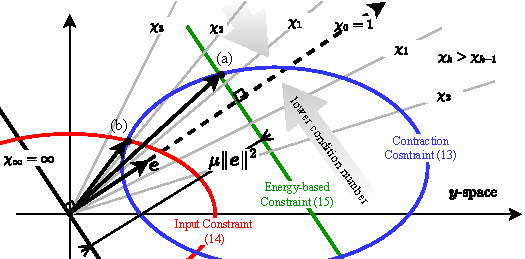
\includegraphics[width=0.99\linewidth]
   {
      figures/scene_first.drawio.pdf
   }
   \caption{
      Illustration of the optimization problem \eqref{eq:opt:main} in two-dimensional space; see Section~\ref{sec:sub:illustrative} for details.
   }
\label{fig:scene:first}
\end{figure}

To facilitate geometric interpretation, the optimization problem \eqref{eq:opt:main} is illustrated in two-dimensional space in Fig.~\ref{fig:scene:first}.
The contraction constraint \eqref{eq:cstr:ctrc:proj} and the input saturation constraint \eqref{eq:cstr:sat} restrict the feasible space of $\mv{y}$ to the outside of the blue line and the inside of the red line, respectively.
The green line represents the energy-based constraint \eqref{eq:cstr:energy}, assuming that the allowable energy variation $\epsilon$ is approximately zero.

Since the contraction constraint \eqref{eq:cstr:ctrc:proj} is an ellipse-shaped concave function and the input saturation constraint \eqref{eq:cstr:sat} is a convex function, there exist at most two intersection points of these constraints.
If the initial guess is set near point (a), the optimal solution converges to point (a), neglecting the input saturation constraint according to the objective function, \ie the minimum angle between $\mv{y}$ and $\mv{e}$.
Considering the input saturation constraint, the optimal solution is obtained at point (b) by increasing the slack variable $s$, which relaxes the energy-based constraint \eqref{eq:cstr:energy} to satisfy the input saturation constraint.

\section{Numerical Validation} \label{sec:validation}

\subsection{Numerical Validation Set Up}

We employed the Lorenz system to validate the proposed method, which is represented as follows:
\begin{equation}
   \ddtt
   \underbrace{
      \begin{pmatrix}
         x\\y\\z
      \end{pmatrix}
   }_{=:\mv{x}}
   =
   \underbrace{
      \begin{pmatrix}
         \sigma(y-x)
         \\
         x(\rho-z)-y
         \\
         xy-\beta z
      \end{pmatrix}
   }_{=:\mv{f}(\mv{x})}
   +
   \mysat
   \bigg(
      \underbrace{
         \begin{pmatrix}
            u_x\\u_y\\u_z
         \end{pmatrix}
      }_{=:\mv{u}}
   \bigg)
   +
   % \underbrace{
   %    \begin{pmatrix}
   %       d_x\\d_y\\d_z
   %    \end{pmatrix}
   % }_{=:\mv{d}}
   \mv{d}(t)
   ,
\end{equation}
where $\sigma=10$, $\rho=28$, and $\beta=\tfrac{8}{3}$ are system parameters.
The input saturation function $\mysat(\cdot)$ was defined as follows:
\begin{equation}
   \mysat(\mv{u})
   :=
   \begin{cases}
      \mv{u}
      ,
      & \text{if } \norm{\mv{u}} \le \overline{u}
      ,
      \\
      \overline{u} \tfrac{\mv{u}}{\norm{\mv{u}}}
      ,
      & \text{otherwise}
      ,
   \end{cases}
\end{equation}
where $\overline{u}=200$ denotes the maximum input magnitude.
The external disturbances $\mv{d}(t)$ were modeled as follows:
\begin{equation}
   \mv{d}(t)
   :=
   1000 (H(t-0.1)-H(t-0.11))
   \cdot
   \mv{1}_{3\times1}
   ,
\end{equation}
where $H(\cdot)$ denotes the Heaviside step function.

For the desired trajectory, we simulated the desired system \eqref{eq:sys:desired} with the desired feedback-linearization control input
% \begin{equation}
$
   \mv{u}_d
   :=
   -\mv{f}(\mv{x}_d) - 2(\mv{x}_d - \mv{r})
   ,
$
% \end{equation}
where $\mv{r}:=(-8.485,8.485,27)^\top$ denotes the reference point.
The desired input was designed not to exceed the input saturation limit.

The proposed method (C$_1$) was compared with CV-STEM (C$_2$) \cite{Tsukamoto:2021ae} and the desired controller, \ie $\mv{u}=\mv{u}_d$, (C$_3$) as summarized in Table~\ref{table:controllers}.
The parameters shared by (C$_1$) and (C$_2$) were $\alpha=10$ and $\mm{R}=\mm{I}_3$.
In addition, parameters were selected as $\mu=30$ and $\lambda=500$ for (C$_1$) and $\lambda=1e-10$ for (C$_2$).
To solve the optimization problems, the \texttt{fmincon} function and \texttt{SeMeDi} toolbox were used for (C$_1$) and (C$_2$) in MATLAB R2024b, respectively.

\begin{table}[t]
   \renewcommand{\arraystretch}{1.3}
   \caption{Controllers for comparative study.}
   \centering
   % \begin{tabular}{c m{13.5em}}
   \begin{tabular}{c l}
   \hline
   & \textbf{Description} \\
   \hline
   \hline 
   (C$_1$) \protect\colorLine{blue}{solid} & Proposed controller. \\ 
   \hline
   (C$_2$) \protect\colorLine{my_cyan}{solid} & CV-STEM (\cite{Tsukamoto:2021ae}). \\
   \hline
   (C$_3$) \protect\colorLine{gray}{solid} & Desired controller, \ie $\mv{u}=\mv{u}_d$. \\
   \hline
   \end{tabular}
   \label{table:controllers}
\end{table}

The simulation was conducted for $T=0.5$ seconds with a sampling time of $T_s=0.005$ seconds for the controllers and a $10$ times finer time step for the system simulation.
The initial conditions were set to $\mv{x}(0)=(10,5,13)^\top$ and $\mv{x}_d(0)=(11,4,15)^\top$.

To facilitate reproducibility, the numerical validation source code is publicly available at \url{https://github.com/KAIST-MIC-Lab/Deep-Neuro-Control}

\subsection{Numerical Validation Results}

\begin{figure}[t]
   \centering
   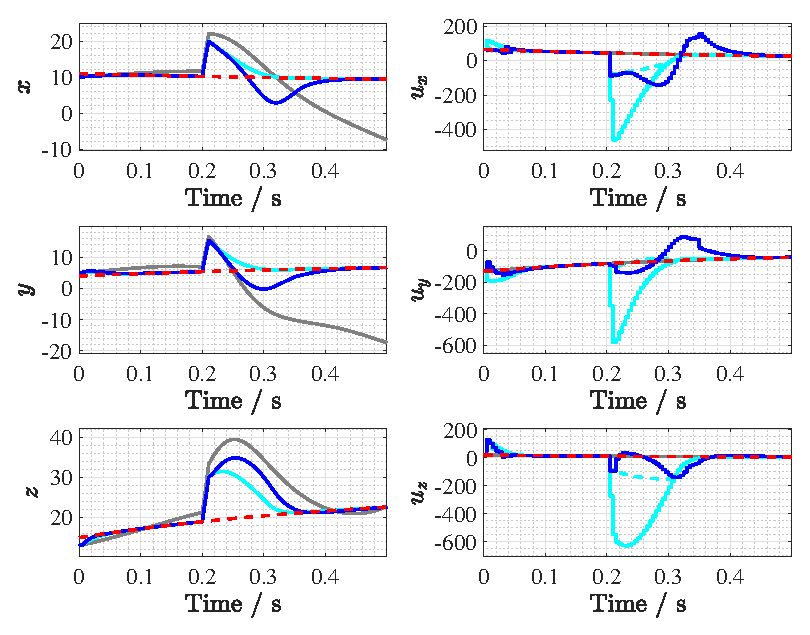
\includegraphics[width=0.99\linewidth]
   {
      src/script_simulation/figures/compare/Fig1.eps
   }
   \caption{
      Numerical validation results of (C$_1$) \protect\colorLine{blue}{solid}, (C$_2$) \protect\colorLine{my_cyan}{solid}, (C$_3$) \protect\colorLine{gray}{solid}, and desired trajectory $x_d$ \protect\colorLine{red}{dashed}.
      The dashed line indicates the saturated input in the figures on the right-hand side.
   }
   \label{fig:sim:result:control}
\end{figure}

\begin{figure}[t]
   \centering
   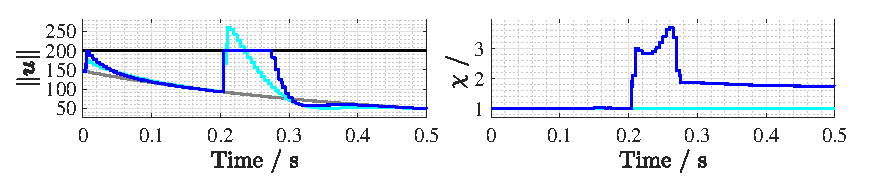
\includegraphics[width=0.99\linewidth]
   {
      src/script_simulation/figures/compare/Fig2.eps
   }
   \caption{
      Control input norms, condition numbers, penalty term, and slack variable of (C$_1$) \protect\colorLine{blue}{solid}, (C$_2$) \protect\colorLine{my_cyan}{solid}, and (C$_3$) \protect\colorLine{gray}{solid}.
   }
   \label{fig:sim:result:opt}
\end{figure}

\begin{table}[t]
   \renewcommand{\arraystretch}{1.3}
   \caption{Tracking performances in $L_2$ norm.}
   \centering
   \begin{tabular}{c c c c }
   % \begin{tabular}{c c c c c}
   \hline
   & (C$_1$) \protect\colorLine{blue}{solid} & (C$_2$) \protect\colorLine{my_cyan}{solid} & (C$_3$) \protect\colorLine{gray}{solid} \\
   \hline
   \hline 
   % \multirow{2}{*}{
   $\int_0^T\norm{\mv{e}}\,\der t$
   % } 
   & \oneErr & \twoErr & \threeErr \\
   % & (-\impOne \%)  & (-\impTwo \%) & (–) \\
   \hline
   \end{tabular}
   \label{table:performance}
\end{table}

The numerical validation results are illustrated in Figs.~\ref{fig:sim:result:control} and \ref{fig:sim:result:opt}.
When only the desired controller was applied, \ie (C$_3$), the trajectories of (C$_3$) and $\mv{x}_d$ do not coincide due to the effect of initial condition mismatch.
Significantly, after the disturbance occurrence at $t=0.2$ seconds, the trajectory deviates further from the desired trajectory, as shown in Fig.~\ref{fig:sim:result:control}.

By applying the contraction-based controllers, both (C$_1$) and (C$_2$) successfully drive the trajectory to closely follow the desired trajectory $\mv{x}_d$ even in the presence of disturbances, minimizing the $L_2$ norm of the tracking error to {\oneErr} and {\twoErr}, while (C$_3$) resulted in {\threeErr}, as summarized in Table~\ref{table:performance}.
However, regarding input saturation, (C$_2$) reaches the saturation limit due to the initial condition mismatch and the disturbance at $t=0.2$, while (C$_1$) effectively avoids input saturation, as shown in Fig.~\ref{fig:sim:result:opt}.
This demonstrates the effectiveness of the proposed method in handling input saturation constraints while achieving satisfactory tracking performance.

In addition, the expected behavior of the condition number $\chi$ of the contraction metrics, discussed in Section~\ref{sec:main:illustrative} and Fig.~\ref{fig:scene:first}, can be observed for (C$_1$) in Fig.~\ref{fig:sim:result:opt}.
As the contraction constraint \eqref{eq:cstr:ctrc} and the input saturation constraint \eqref{eq:cstr:sat} become active, the angle between $\mv{y}$ and $\mv{e}$ increases, resulting in an increase in the condition number to find an unsaturated optimal solution.
Specifically, when the input saturation constraint became active, the condition number $\chi$ increased from $1$ and decreased again to $1$ after the saturation effect disappeared.

In contrast, (C$_2$) shows the smallest condition number, $\chi=1$, due to the problem formulation issue discussed in Remark~\ref{rem:scale:invariance}.
Instead of adjusting the condition number, (C$_2$) increases the penalty term $\nu$ to increase the control effort, as shown in Fig.~\ref{fig:sim:result:opt}, while making $\overline{W}$ close to the identity matrix, \ie $\mm{M}=\nu\mm{I}_n$.
This results in the failure to satisfy the contraction constraint \eqref{eq:cstr:ctrc} during most of the simulation time, as shown in Fig.~\ref{fig:sim:result:opt}.

\section{Conclusion} \label{sec:conclusion}

In this study, we presented a vector-space optimization framework for contraction metric calculation in contraction theory-based control design.
By projecting the contraction constraints onto the trajectory error vector space, the contraction metrics can be calculated in a lower-dimensional effective space, resolving the scalability issue of the conventional LMI framework.
The optimization problem was formulated to minimize the condition number of the contraction metric, where energy-based constraints were introduced to resolve the scale-invariance ambiguity and ensure sufficient control effort. 
Additionally, convex input saturation constraints were easily incorporated into the proposed framework owing to its flexibility compared to the conventional LMI framework.
As future work, we will extend the proposed method to handle state constraints and validate it through real-world experiments.

% \begin{ack}
% Place acknowledgments here.
% \end{ack}

\bibliography{template/refs, localRefs}             % bib file to produce the bibliography
                                    % with bibtex (preferred)
\end{document}